\section{Question 3}

\textbf{\textit{Assuming a raised male voice in the conference room, calculate the sound pressure level in the adjacent single office due to sound transmission through both the ductwork and the common partition.}}


The resolution of the SPL in the single office due to the sound transmission of a raised male voice through the ductwork and partition, L\textsubscript{p\textsubscript{male\textsubscript{2}}}, is detailed at 63~Hz in Table~\ref{tbl:SPL_office_example} and further explained below.



\subsection{Step 1: Male voice SPL in conference room}

The first step is to calculate the SPL of the raised male voice in the conference room, L\textsubscript{p\textsubscript{male\textsubscript{1}}}.
This is done by using Equation~\ref{eq:SPL}.
V\textsubscript{1} is found in Table~\ref{tbl:room_dims} and the other variables are detailed in Table~\ref{tbl:SPL_office_example}.



\subsection{Step 2: Sound transmission through a single ductwork}

The second step is to calculate the SPL in the single office due to the sound transmission of the male voice through a single ductwork, L\textsubscript{p\textsubscript{male\textsubscript{2}duct}}.
This has been done in the following manner:
\begin{itemize}
	\item The sound power level entering the duct is calculated using Equation~\ref{eq:power_in}, where L\textsubscript{p} is the SPL in the source room and S is the cross-sectional area of the duct.
		\begin{equation}\label{eq:power_in}
			L_{W in} = L_{p} + 10 log \frac{S}{4}
		\end{equation}
	\item From the conference room to the single office, the man's voice is attenuated six times, as listed below. The calculations of these attenuations are detailed in Table~\ref{tbl:SPL_office_example}.
		\begin{enumerate}
			\item Along the 0.5~m vertical duct
			\item At the branch
			\item Along the 4~m horizontal duct
			\item At the branch
			\item Along the 0.5~m vertical duct
			\item At the duct termination due to end reflection losses
		\end{enumerate}
	\item The sound power level leaving a single ductwork is calculated using Equation~\ref{eq:power_out}.
	\item The SPL in the single office due to the sound transmission of the male voice through a single ductwork, L\textsubscript{p\textsubscript{male\textsubscript{2}duct}}, is calculated using Equation~\ref{eq:SPL}. For this, V\textsubscript{2} is found in Table~\ref{tbl:room_dims}.
\end{itemize}



\subsection{Step 3: Sound transmission through the partition}

The third step is to calculate the SPL in the single office due to the sound transmission of the male voice through the partition, L\textsubscript{p\textsubscript{male\textsubscript{2}partition}}.
For this we re-arrange the Sound Reduction Index (SRI) formula (Equation~\ref{eq:SRI}) to find L\textsubscript{p\textsubscript{male\textsubscript{2}partition}} (Equation~\ref{eq:SRI_rearranged}).
Note that S in Equations~\ref{eq:SRI} and \ref{eq:SRI_rearranged} is the surface area of the common wall in square metres.

	\begin{equation}\label{eq:SRI}
		R = L_1 - L_2 + 10 log \frac{S}{A_2}
	\end{equation}
	
	
	\begin{equation}\label{eq:SRI_rearranged}
		L_2 = L_1 - R + 10 log \frac{S}{A_2}
	\end{equation}

\begin{itemize}
	\item The SRI values of the partition, R, are given in Table~2 of the assignment description.
	\item The surface area of the partition wall, S\textsubscript{partition}, is found in Table~\ref{tbl:room_dims}.
	\item The absorption of the single office, A\textsubscript{2}, is found in Table~\ref{tbl:reverb_office}.
\end{itemize}

The calculation of L\textsubscript{p\textsubscript{male\textsubscript{2}partition}} is detailed in Table~\ref{tbl:SPL_office_example}.



\subsection{Step 4: Sound transmission through partition and both ducts}

The final step is to sum the SPLs in the office due to sound transmission through the partition and both the supply and return ducts.
For this we use Equation~\ref{eq:sum} to calculate the sum of any number of levels.
See detailed calculation of L\textsubscript{p\textsubscript{male\textsubscript{2}}} in Table~\ref{tbl:SPL_office_example}.

	\begin{equation}\label{eq:sum}
		L_T = 10 log \left(10^{L_1/10} + 10^{L_2/10} + 10^{L_3/10} + \ldots\right) = 10 log \left(\sum_{i}10^{L_i/10}\right)
	\end{equation}



\subsection{L\textsubscript{p\textsubscript{male\textsubscript{2}}} results at all frequencies}

Table~\ref{tbl:SPL_office} presents the L\textsubscript{p\textsubscript{male\textsubscript{2}}} results in octave bands between 63~Hz and 4~kHz.

The chart in Figure~\ref{fig:Lpmale} presents the SPLs of the raised male voice in the conference room and in the single office due to sound transmission through the ductwork, partition, and both the ductwork and partition.

% Please add the following required packages to your document preamble:
% \usepackage{booktabs}
\begin{sidewaystable}[htbp]
	\caption{Details of the calculation of the SPL in the single office due to sound transmission of a raised male voice through the ductwork and partition, L\textsubscript{p\textsubscript{male\textsubscript{2}}}, at 63~Hz.}
	\label{tbl:SPL_office_example}
	\centering
	\begin{tabular}{@{}l@{\hspace*{0.5em}}lrm{10.5cm}@{}}% <-- @{} adjusted inter column space
		\toprule
		Step & Frequency (Hz) & 63 & Notes \\ \midrule
		\multirow{5}{*}{1 \vastt\{ } & L\textsubscript{W\textsubscript{male}} (dB re 10\textsuperscript{-12} W) & 62.29 & Read off the chart in Table~7 of assignment description \\
		& & \multicolumn{1}{l}{} &  \\
		& T\textsubscript{1} (s) & 0.48 & From Table~\ref{tbl:reverb_conf} \\
		& & \multicolumn{1}{l}{} &  \\
		& L\textsubscript{p\textsubscript{male\textsubscript{1}}} (dB) & $62.29 - 10 log \left(\frac{80}{0.48}\right) + 14 = 54.11$ & \begin{tabular}[c]{@{}l@{}}SPL in conference room due to man's voice:\\ $L_{p_{male_1}} = L_{W male} – 10 log \frac{V_1}{T_1} + 14$\end{tabular} \\
		& & \multicolumn{1}{l}{} &  \\
		\multirow{21}{*}{2 \Vastt\{ } & L\textsubscript{W\textsubscript{in}} (dB re 10\textsuperscript{-12} W) & $54.11 + 10 log \left(\frac{0.12}{4}\right) = 38.88$ & \begin{tabular}[c]{@{}l@{}}Sound power level entering single ductwork:\\ $L_{W in} = L_{p_{male_1}} + 10 log \frac{S_{vertical}}{4}$\end{tabular} \\
		& & \multicolumn{1}{l}{} &  \\
		& Attn\textsubscript{vertical} (dB) & $0.5 \times (1 + 1) = 1.00$ & Same as notes for Attn\textsubscript{vertical} in Table~\ref{tbl:BN_conf_example} \\
		& & \multicolumn{1}{l}{} &  \\
		& Attn\textsubscript{vertical $\rightarrow$ horizontal} (dB) & $\left|10 log \frac{0.24}{0.24 + 0.24}\right| = 3.01$ & $\left|10 log \frac{S_{horizontal}}{S_{horizontal} + S_{horizontal}}\right|$ \\
		& & \multicolumn{1}{l}{} &  \\
		& Attn\textsubscript{horizontal} (dB) & $4 \times (1 + 1.64) = 10.56$ & Same as notes for Attn\textsubscript{horizontal} in Table~\ref{tbl:BN_conf_example} but for a duct length of 4~m \\
		& & \multicolumn{1}{l}{} &  \\
		& Attn\textsubscript{horizontal $\rightarrow$ vertical} (dB) & $\left|10 log \frac{0.12}{0.12 + 0.24}\right| = 4.77$ & $\left|10 log \frac{S_{vertical}}{S_{vertical} + S_{horizontal}}\right|$ \\
		& & \multicolumn{1}{l}{} &  \\
		& Attn\textsubscript{vertical} (dB) & $0.5 \times (1 + 1) = 1.00$ & Same as notes for Attn\textsubscript{vertical} in Table~\ref{tbl:BN_conf_example} \\
		& & \multicolumn{1}{l}{} &  \\
		& Attn\textsubscript{end reflections} (dB) & 11 & Given in Table~6 of assignment description for a duct cross-sectional area of 0.3~m $\times$ 0.4~m = 0.12~m\textsuperscript{2} \\
		& & \multicolumn{1}{l}{} &  \\
		& $\Sigma$Attn (dB) & 31.34 & Sum of all attenuations \\
		& & \multicolumn{1}{l}{} &  \\
		& L\textsubscript{W\textsubscript{out}} (dB re 10\textsuperscript{-12} W) & $38.88 - 31.34 = 7.53$ & \begin{tabular}[c]{@{}l@{}}Sound power level leaving single ductwork: $L_{W out} = L_{W in} - \Sigma Attn$\end{tabular} \\
		& & \multicolumn{1}{l}{} &  \\
		& T\textsubscript{2} (s) & 0.47 & From Table~\ref{tbl:reverb_office} \\
		& & \multicolumn{1}{l}{} &  \\
		& L\textsubscript{p\textsubscript{male\textsubscript{2}duct}} (dB) & $7.53 - 10 log \left(\frac{50}{0.47}\right) + 14 = 1.26$ & \begin{tabular}[c]{@{}l@{}}SPL in office due to man's voice: $L_{p_{male_2duct}} = L_{W out} – 10 log \frac{V_2}{T_2} + 14$\end{tabular} \\
		& & \multicolumn{1}{l}{} &  \\
		\multirow{5}{*}{3 \vastt\{ } & R (dB) & 20 & Given in Table~2 of assignment description \\
		& & \multicolumn{1}{l}{} &  \\
		& A\textsubscript{2} (s) & 17.15 & From Table~\ref{tbl:reverb_office} \\
		& & \multicolumn{1}{l}{} &  \\
		& L\textsubscript{p\textsubscript{male\textsubscript{2}partition}} (dB) & $54.11 - 20 + 10 log \left(\frac{10}{17.15}\right) = 31.76$ & \begin{tabular}[c]{@{}l@{}}Re-arrange SRI formula to get SPL after partition:\\ $L_{p_{male_2partition}} = L_{p_{male_1}} – R + 10 log \frac{S_{partition}}{A_2}$\end{tabular} \\
		& & \multicolumn{1}{l}{} &  \\
		4 & L\textsubscript{p\textsubscript{male\textsubscript{2}}} (dB) & $10 log \left(10^{1.26/10} + 10^{1.26/10} + 10^{31.76/10}\right) = 31.8$ & Sum of three SPLs: through supply duct, return duct and partition \\ \bottomrule
	\end{tabular}
\end{sidewaystable}

% Please add the following required packages to your document preamble:
% \usepackage{booktabs}
\begin{table}[htbp]
	\caption{Calculation of the SPL in the single office due to sound transmission of a raised male voice through the ductwork and partition, L\textsubscript{p\textsubscript{male\textsubscript{2}}}.}
	\label{tbl:SPL_office}
	\centering
	\begin{tabular}{@{}l@{\hspace*{0.5em}}lrrrrrrr@{}}% <-- @{} adjusted inter column space
		\toprule
		Step & Frequency (Hz) & 63 & 125 & 250 & 500 & 1000 & 2000 & 4000 \\ \midrule
		\multirow{3}{*}{1 \vast\{ } & L\textsubscript{W\textsubscript{male}} (dB re 10\textsuperscript{-12} W) & 62.29 & 67.43 & 70.00 & 73.53 & 74.71 & 70.00 & 60.00 \\
		& T\textsubscript{1} (s) & 0.48 & 0.44 & 0.47 & 0.49 & 0.37 & 0.32 & 0.30 \\
		& L\textsubscript{p\textsubscript{male\textsubscript{1}}} (dB) & 54.11 & 58.78 & 61.70 & 65.41 & 65.34 & 59.99 & 49.79 \\
		\multirow{11}{*}{2 \Vast\{ } & L\textsubscript{W\textsubscript{in}} (dB re 10\textsuperscript{-12} W) & 38.88 & 43.56 & 46.47 & 50.18 & 50.11 & 44.76 & 34.56 \\
		& Attn\textsubscript{vertical} (dB) & 1.00 & 1.32 & 1.00 & 0.66 & 0.23 & 0.23 & 0.23 \\
		& Attn\textsubscript{vertical $\rightarrow$ horizontal} (dB) & 3.01 & 3.01 & 3.01 & 3.01 & 3.01 & 3.01 & 3.01 \\
		& Attn\textsubscript{horizontal} (dB) & 10.56 & 10.56 & 6.64 & 3.92 & 1.56 & 1.56 & 1.56 \\
		& Attn\textsubscript{horizontal $\rightarrow$ vertical} (dB) & 4.77 & 4.77 & 4.77 & 4.77 & 4.77 & 4.77 & 4.77 \\
		& Attn\textsubscript{vertical} (dB) & 1.00 & 1.32 & 1.00 & 0.66 & 0.23 & 0.23 & 0.23 \\
		& Attn\textsubscript{end reflections} (dB) & 11 & 7 & 3 & 1 & 0 & 0 & 0 \\
		& $\Sigma$Attn (dB) & 31.34 & 27.98 & 19.42 & 14.02 & 9.80 & 9.80 & 9.80 \\
		& L\textsubscript{W\textsubscript{out}} (dB re 10\textsuperscript{-12} W) & 7.53 & 15.57 & 27.05 & 36.16 & 40.31 & 34.96 & 24.76 \\
		& T\textsubscript{2} (s) & 0.47 & 0.41 & 0.46 & 0.48 & 0.36 & 0.31 & 0.30 \\
		& L\textsubscript{p\textsubscript{male\textsubscript{2}duct}} (dB) & 1.26 & 8.70 & 20.65 & 29.96 & 32.91 & 26.92 & 16.52 \\
		\multirow{3}{*}{3 \vast\{ } & R (dB) & 20 & 32 & 45 & 52 & 58 & 64 & 61 \\
		& A\textsubscript{2} (s) & 17.15 & 19.70 & 17.65 & 16.85 & 22.25 & 25.80 & 27.00 \\
		& L\textsubscript{p\textsubscript{male\textsubscript{2}partition}} (dB) & 31.76 & 23.84 & 14.23 & 11.14 & 3.87 & -8.12 & -15.52 \\
		4 & L\textsubscript{p\textsubscript{male\textsubscript{2}}} (dB) & 31.8 & 24.1 & 24.1 & 33.0 & 35.9 & 29.9 & 19.5 \\ \bottomrule
	\end{tabular}
\end{table}

\begin{figure}[htbp]
	\centering
	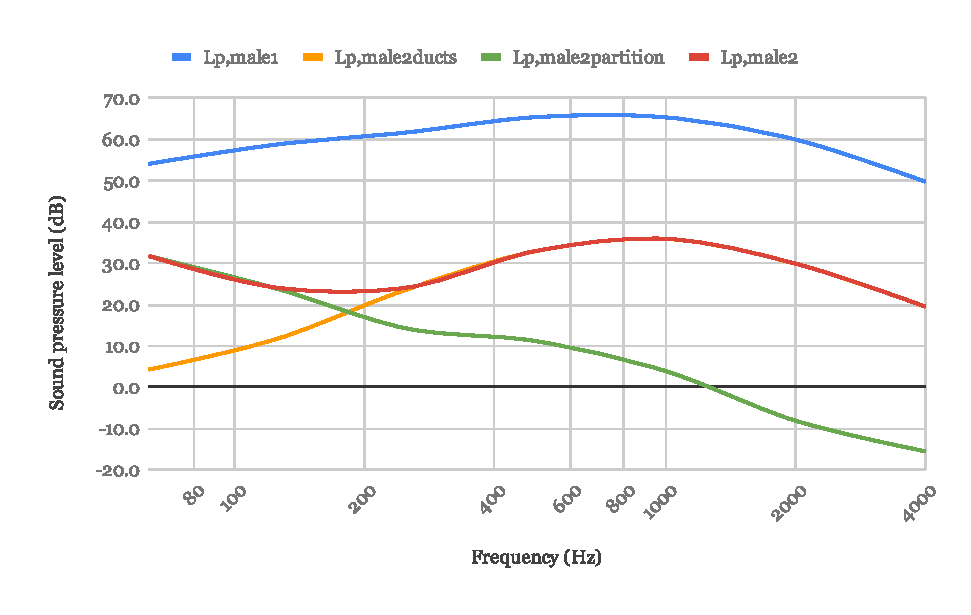
\includegraphics[width=\textwidth]{figures/Lpmale.eps}
	\rule{\textwidth}{0.5pt} % use line???
	\caption{The SPLs of the raised male voice in the conference room (L\textsubscript{p\textsubscript{male\textsubscript{1}}}) and in the single office due to sound transmission through the ductwork (L\textsubscript{p\textsubscript{male\textsubscript{2}ducts}}), partition (L\textsubscript{p\textsubscript{male\textsubscript{2}partition}}) and both (L\textsubscript{p\textsubscript{male\textsubscript{2}}}).}
	\label{fig:Lpmale}
\end{figure}